\documentclass[conference]{IEEEtran}
\usepackage{amsmath,amssymb,graphicx,booktabs,xcolor,url,cite,array}
\usepackage[hidelinks]{hyperref}
\graphicspath{{figures/}{../results/v2_samplerfix/}}
% generated by draft1/make_numbers.py -- do not edit
\newcommand{\NRegDossiers}{500}
\newcommand{\NRegTurns}{3000}
\newcommand{\NRegH}{186}
\newcommand{\NRegU}{342}
\newcommand{\NRegG}{2471}
\newcommand{\RegHpct}{6.2}
\newcommand{\RegGpct}{82.4}
\newcommand{\RegUpct}{11.4}
\newcommand{\NRegOnset}{135}
\newcommand{\NRegWrong}{64}
\newcommand{\NRegMissCode}{110}
\newcommand{\NRegInvented}{12}
\newcommand{\NClinDossiers}{300}
\newcommand{\NClinTurns}{1800}
\newcommand{\NClinH}{56}
\newcommand{\NClinU}{167}
\newcommand{\NClinG}{1577}
\newcommand{\ClinHpct}{3.1}
\newcommand{\ClinGpct}{87.6}
\newcommand{\ClinUpct}{9.3}
\newcommand{\NClinOnset}{44}
\newcommand{\NClinWrong}{24}
\newcommand{\NClinMissCode}{32}
\newcommand{\NClinInvented}{0}
\newcommand{\PilotVone}{0.0}
\newcommand{\PilotVtwo}{6.9}
\newcommand{\PrimRegL}{-0.034\,[-0.079,\,+0.015]}
\newcommand{\OnsetsRegL}{24}
\newcommand{\AucMzeroRegL}{0.755\,[0.640,\,0.859]}
\newcommand{\AucMoneRegL}{0.712\,[0.586,\,0.825]}
\newcommand{\AucMtwoRegL}{0.678\,[0.561,\,0.788]}
\newcommand{\AucMthreeRegL}{0.669\,[0.555,\,0.782]}
\newcommand{\AucMfourRegL}{0.836\,[0.752,\,0.908]}
\newcommand{\RhatMthreeRegL}{1.875}
\newcommand{\EssMthreeRegL}{6}
\newcommand{\RhatPreMthreeRegL}{2.345}
\newcommand{\EssPreMthreeRegL}{5}
\newcommand{\RhatMfourRegL}{1.663}
\newcommand{\EssMfourRegL}{6}
\newcommand{\RhatPreMfourRegL}{2.403}
\newcommand{\EssPreMfourRegL}{5}
\newcommand{\EvidRegL}{-0.033\,[-0.069,\,-0.008]}
\newcommand{\AmbRegL}{+0.001\,[-0.020,\,+0.033]}
\newcommand{\AmbPRegL}{0.52}
\newcommand{\HtwoPRegL}{0.0005}
\newcommand{\HtwoObsRegL}{27}
\newcommand{\HtwoNullRegL}{9.8}
\newcommand{\WithinPRegL}{0.159}
\newcommand{\WithinInfRegL}{35}
\newcommand{\BrierMthreeRegL}{-0.0003\,[-0.0007,\,+0.0001]}
\newcommand{\BrierBaseRegL}{+0.0004\,[-0.0004,\,+0.0011]}
\newcommand{\PrimRegX}{-0.008\,[-0.035,\,+0.021]}
\newcommand{\OnsetsRegX}{24}
\newcommand{\AucMzeroRegX}{0.755\,[0.640,\,0.859]}
\newcommand{\AucMoneRegX}{0.781\,[0.651,\,0.888]}
\newcommand{\AucMtwoRegX}{0.772\,[0.648,\,0.885]}
\newcommand{\AucMthreeRegX}{0.773\,[0.647,\,0.879]}
\newcommand{\AucMfourRegX}{0.820\,[0.716,\,0.906]}
\newcommand{\RhatMthreeRegX}{1.001}
\newcommand{\EssMthreeRegX}{2651}
\newcommand{\RhatPreMthreeRegX}{1.529}
\newcommand{\EssPreMthreeRegX}{7}
\newcommand{\RhatMfourRegX}{1.439}
\newcommand{\EssMfourRegX}{143}
\newcommand{\RhatPreMfourRegX}{1.047}
\newcommand{\EssPreMfourRegX}{105}
\newcommand{\EvidRegX}{-0.073\,[-0.129,\,-0.020]}
\newcommand{\AmbRegX}{+0.026\,[-0.023,\,+0.087]}
\newcommand{\AmbPRegX}{0.82}
\newcommand{\HtwoPRegX}{0.0005}
\newcommand{\HtwoObsRegX}{27}
\newcommand{\HtwoNullRegX}{9.8}
\newcommand{\WithinPRegX}{0.159}
\newcommand{\WithinInfRegX}{35}
\newcommand{\BrierMthreeRegX}{+0.0040\,[+0.0027,\,+0.0050]}
\newcommand{\BrierBaseRegX}{-0.0060\,[-0.0102,\,-0.0010]}
\newcommand{\PrimClinL}{-0.102\,[-0.208,\,-0.002]}
\newcommand{\OnsetsClinL}{8}
\newcommand{\AucMzeroClinL}{0.797\,[0.672,\,0.916]}
\newcommand{\AucMoneClinL}{0.844\,[0.778,\,0.912]}
\newcommand{\AucMtwoClinL}{0.742\,[0.591,\,0.885]}
\newcommand{\AucMthreeClinL}{0.810\,[0.657,\,0.948]}
\newcommand{\AucMfourClinL}{0.842\,[0.630,\,0.963]}
\newcommand{\RhatMthreeClinL}{1.590}
\newcommand{\EssMthreeClinL}{7}
\newcommand{\RhatPreMthreeClinL}{1.992}
\newcommand{\EssPreMthreeClinL}{5}
\newcommand{\RhatMfourClinL}{1.385}
\newcommand{\EssMfourClinL}{9}
\newcommand{\RhatPreMfourClinL}{1.426}
\newcommand{\EssPreMfourClinL}{8}
\newcommand{\EvidClinL}{-0.011\,[-0.057,\,+0.011]}
\newcommand{\AmbClinL}{+0.005\,[-0.007,\,+0.027]}
\newcommand{\AmbPClinL}{0.78}
\newcommand{\HtwoPClinL}{0.0020}
\newcommand{\HtwoObsClinL}{6}
\newcommand{\HtwoNullClinL}{1.5}
\newcommand{\WithinPClinL}{0.447}
\newcommand{\WithinInfClinL}{9}
\newcommand{\BrierMthreeClinL}{+0.0153\,[+0.0112,\,+0.0182]}
\newcommand{\BrierBaseClinL}{-0.0004\,[-0.0007,\,+0.0001]}
\newcommand{\PrimClinX}{-0.001\,[-0.004,\,+0.001]}
\newcommand{\OnsetsClinX}{8}
\newcommand{\AucMzeroClinX}{0.797\,[0.672,\,0.916]}
\newcommand{\AucMoneClinX}{0.844\,[0.732,\,0.943]}
\newcommand{\AucMtwoClinX}{0.843\,[0.730,\,0.942]}
\newcommand{\AucMthreeClinX}{0.826\,[0.624,\,0.963]}
\newcommand{\AucMfourClinX}{0.821\,[0.600,\,0.965]}
\newcommand{\RhatMthreeClinX}{1.001}
\newcommand{\EssMthreeClinX}{3053}
\newcommand{\RhatPreMthreeClinX}{1.723}
\newcommand{\EssPreMthreeClinX}{6}
\newcommand{\RhatMfourClinX}{1.386}
\newcommand{\EssMfourClinX}{146}
\newcommand{\RhatPreMfourClinX}{1.521}
\newcommand{\EssPreMfourClinX}{40}
\newcommand{\EvidClinX}{-0.092\,[-0.159,\,-0.024]}
\newcommand{\AmbClinX}{+0.053\,[+0.006,\,+0.124]}
\newcommand{\AmbPClinX}{0.99}
\newcommand{\HtwoPClinX}{0.0020}
\newcommand{\HtwoObsClinX}{6}
\newcommand{\HtwoNullClinX}{1.5}
\newcommand{\WithinPClinX}{0.447}
\newcommand{\WithinInfClinX}{9}
\newcommand{\BrierMthreeClinX}{-0.0032\,[-0.0038,\,-0.0024]}
\newcommand{\BrierBaseClinX}{-0.0075\,[-0.0106,\,-0.0037]}
\newcommand{\PHgivenH}{17.2}
\newcommand{\PHgivenNotH}{5.5}
\newcommand{\PosOnlyP}{2.3\times10^{-90}}
\newcommand{\DiffOnlyP}{0.463}
\newcommand{\CorrReg}{-0.120\,[-0.182,\,-0.070]}
\newcommand{\CorrBetterReg}{15}
\newcommand{\CorrWorseReg}{0}
\newcommand{\CorrSignReg}{6.1e-05}
\newcommand{\RegrReg}{-0.037\,[-0.093,\,+0.012]}
\newcommand{\RegrUReg}{+0.083}
\newcommand{\IvNReg}{121}
\newcommand{\OrigHReg}{14.5}
\newcommand{\CorrHReg}{2.5}
\newcommand{\CorrClin}{-0.098\,[-0.201,\,-0.028]}
\newcommand{\CorrBetterClin}{4}
\newcommand{\CorrWorseClin}{0}
\newcommand{\CorrSignClin}{0.12}
\newcommand{\RegrClin}{-0.024\,[-0.090,\,-0.001]}
\newcommand{\RegrUClin}{+0.041}
\newcommand{\IvNClin}{41}
\newcommand{\OrigHClin}{12.2}
\newcommand{\CorrHClin}{2.4}
\newcommand{\GuardSilentU}{2.3}
\newcommand{\GuardSilentG}{0.7}
\newcommand{\GuardHeld}{39}
\newcommand{\GuardHoldRate}{13.0}
\newcommand{\GuardPrec}{0.231}
\newcommand{\GuardRecall}{0.818}
\newcommand{\GuardHU}{2.3}
\newcommand{\GuardHG}{3.7}
\newcommand{\GuardPaired}{+0.013\,[-0.003,\,+0.037]}
\newcommand{\GuardMonCaught}{5}
\newcommand{\GuardMonTotal}{7}
\newcommand{\GuardMonHolds}{31}
\newcommand{\GuardThr}{0.091}
\newcommand{\GuardRegr}{131}
\newcommand{\GuardHHeld}{9}
\newcommand{\GuardHtot}{11}
\newcommand{\AtkClean}{6.1}
\newcommand{\AtkInj}{20.6}
\newcommand{\AtkPress}{8.6}
\newcommand{\AtkPressed}{12.3}
\newcommand{\AtkObey}{49}
\newcommand{\AtkAdopt}{11}
\newcommand{\AtkPressTurns}{146}
\newcommand{\AtkAucInj}{0.81}
\newcommand{\SbcPre}{0.003}
\newcommand{\SbcPost}{0.024}
\newcommand{\CovPre}{0.756}
\newcommand{\CovPost}{0.978}
\newcommand{\StarterFS}{41}
\newcommand{\StarterRhat}{1.71}
\newcommand{\StarterEss}{6}

\begin{document}

\title{Does Conversation History Help Detect the First Hallucination?\\ A Bayesian Hidden-Markov Study of Multi-Turn LLM Answers\\ with a Clinical Guard Application}
\author{\IEEEauthorblockN{Nihar Narsana}
\IEEEauthorblockA{MS Data Science --- Bayesian Inference and Modelling\\ University of Arizona, Tucson, AZ, USA}}
\maketitle

\begin{abstract}
Language models that answer a sequence of questions can give an unsupported answer and then build on it. We ask whether modelling the conversation as a hidden Markov process with grounded (G), uncertain (U) and hallucinating (H) states detects the \emph{first} unsupported answer better than a static detector with identical emissions. A local Qwen3-4B-Instruct model answered six-turn questions about \NRegDossiers{} fictional registry dossiers and \NClinDossiers{} fictional clinical charts. Every answer was graded deterministically against a gold record, never by an LLM judge. We compare exact EM filtering, a conjugate Bayesian HMM sampled by forward-filtering backward-sampling (FFBS) Gibbs, and a covariate-dependent Bayesian HMM whose transitions depend on pre-answer evidence availability, ambiguity, near-duplicate codes and turn. History gives no measurable gain: the paired onset-AUROC difference (filter $-$ matched static) is \PrimRegL{} on registry data. Error clustering is consistent with dossier difficulty (exact count-preserving test, $p=\WithinPRegL$). Missing evidence raises the risk of entering H (risk difference \EvidRegX{}). A randomised branch experiment shows that correcting an earlier wrong answer changes the next-turn hallucination rate by \CorrReg{}. As an application, a Bayesian guard for a medication-reconciliation assistant reduced silent errors from \GuardSilentU\% to \GuardSilentG\% of answers. An adversarial review found and fixed a variance-sampler defect; after the fix the exploratory homogeneous model passes the convergence gate.
\end{abstract}

\begin{IEEEkeywords}
Hallucination detection, hidden Markov models, Bayesian inference, Gibbs sampling, FFBS, input--output HMM, large language models, clinical decision support
\end{IEEEkeywords}

\section{Introduction}
Multi-turn conversations make hallucinations worse: models commit early and fail to recover~\cite{laban2025}, errors propagate to later turns~\cite{halluhard2026}, and an early mistake can snowball~\cite{zhang2024}. A natural idea is to treat the model's reliability as a \emph{latent regime} that evolves over turns and to infer it with a hidden Markov model (HMM)~\cite{rabiner1989}. If regimes persist, the filter's prior from earlier turns should help flag the next unsupported answer.

This paper tests that idea rather than assuming it. Our contributions are:
\begin{enumerate}
\item a controlled, gold-graded six-turn task in two domains, with a pilot-frozen design;
\item a \emph{matched-emission} comparison that isolates the value of history (identical emissions, scaler and state mapping; a negative control reproduces the static detector to $10^{-15}$);
\item fully Bayesian HMMs, including a covariate-dependent (input--output) HMM~\cite{bengio1995}, with explicit priors, convergence diagnostics and simulation-based calibration;
\item a randomised, matched-seed intervention experiment giving causal evidence for eligible prefixes;
\item a clinical guard application, a red-team study, and a documented adversarial review.
\end{enumerate}

\section{Related Work}
Sequential and dialogue-level hallucination has been studied through snowballing~\cite{zhang2024}, multi-turn degradation~\cite{laban2025,halluhard2026}, dialogue benchmarks~\cite{diahalu2024} and uncertainty fluctuation scores such as SpikeScore~\cite{spikescore2026}. Single-answer detectors use semantic entropy~\cite{farquhar2024}, hidden-state probes~\cite{kossen2024} or attention ratios~\cite{chuang2024}. Conformal methods give distribution-free factuality guarantees~\cite{mohri2024}. Covariate-dependent HMMs descend from the IOHMM~\cite{bengio1995}. Bayesian non-homogeneous HMMs with P\'olya--Gamma augmentation~\cite{holsclaw2017} give an exact alternative to the Metropolis step used here. Medical hallucination benchmarks~\cite{pal2023} motivate the clinical application; the incentive argument of~\cite{kalai2025} motivates keeping abstention (U) distinct from hallucination (H).

\section{Task, Data and Labels}
\textbf{Dossiers.} Each fictional dossier lists 6 entities $\times$ 5 code fields. Between 2 and 6 rows are hidden (missing evidence), up to 5 near-duplicate code pairs are planted, and two entities share a surname. Six template questions follow: lookup, prior reference (``that patient's\ldots''), surname plus year, and missing field (correct answer \texttt{UNKNOWN}). The original $4\times4$ design (v1) produced almost no hallucinations in the pilot (\PilotVone\% H in the saved pilot), so the harder v2 design (\PilotVtwo\% H) was frozen \emph{before} the main collection.

\textbf{Generation.} Qwen3-4B-Instruct-2507 (Q4\_K\_M) ran locally via Ollama at temperature 0.7 with a 32-token cap. The tag \texttt{qwen3:4b} is a thinking model and ignored \texttt{think=false}; the instruct tag was used instead. Top-20 token log-probabilities were recorded.

\textbf{Labels.} A deterministic grader assigns G (correct code, or a warranted \texttt{UNKNOWN}), U (\texttt{UNKNOWN} although the row exists), H (a wrong, invented or unsupported code) or P (pending). Registry: \NRegH{} H (\RegHpct\%), \NRegU{} U, with onsets in \NRegOnset{} of \NRegDossiers{} dossiers. Clinical: \NClinH{} H (\ClinHpct\%). Most errors are \emph{real} codes from the wrong row (\NRegWrong{}) or codes given for missing rows (\NRegMissCode{}); invented codes are rare (\NRegInvented{}).

\textbf{Features and covariates.} Per answer, $x_t=(\bar\ell,\bar e,s)$: mean selected-token log-probability, mean top-20 entropy with a residual bucket (a proxy, not full-vocabulary entropy), and maximum bag-of-words cosine to a visible row. The pre-answer covariates $c_t$ are evidence present, number of matching entities, near-duplicate load and turn. All are computable from the visible chart and the question alone.

\section{Models}
The three hidden states $z_t\in\{G,U,H\}$ have diagonal Gaussian-mixture emissions:
\begin{equation}
b_j(x)=\sum_{m=1}^{M} w_{jm}\prod_{d=1}^{3}\mathcal N(x_d;\mu_{jmd},v_{jmd}).
\end{equation}
The covariate model (M4) uses softmax transitions with destination H as the reference,
\begin{equation}
A_{ij}(c)=\frac{\exp(\alpha_{ij}+\beta_{ij}^{\top}c)}{\sum_k \exp(\alpha_{ik}+\beta_{ik}^{\top}c)} .
\end{equation}
The causal filter is $f_t\propto b(x_t)\odot f_{t-1}A(c_t)$. We compare: M0, the best single feature (chosen on validation); M1, a \emph{matched static} mixture $s_j(x)\propto\bar\pi_j b_j(x)$ with the same emissions; M2, EM-HMM filtering (3 starts); M3, a Bayesian homogeneous HMM; and M4, a Bayesian covariate HMM. States are mapped to G/U/H on validation labels only.

\begin{figure}[t]\centering
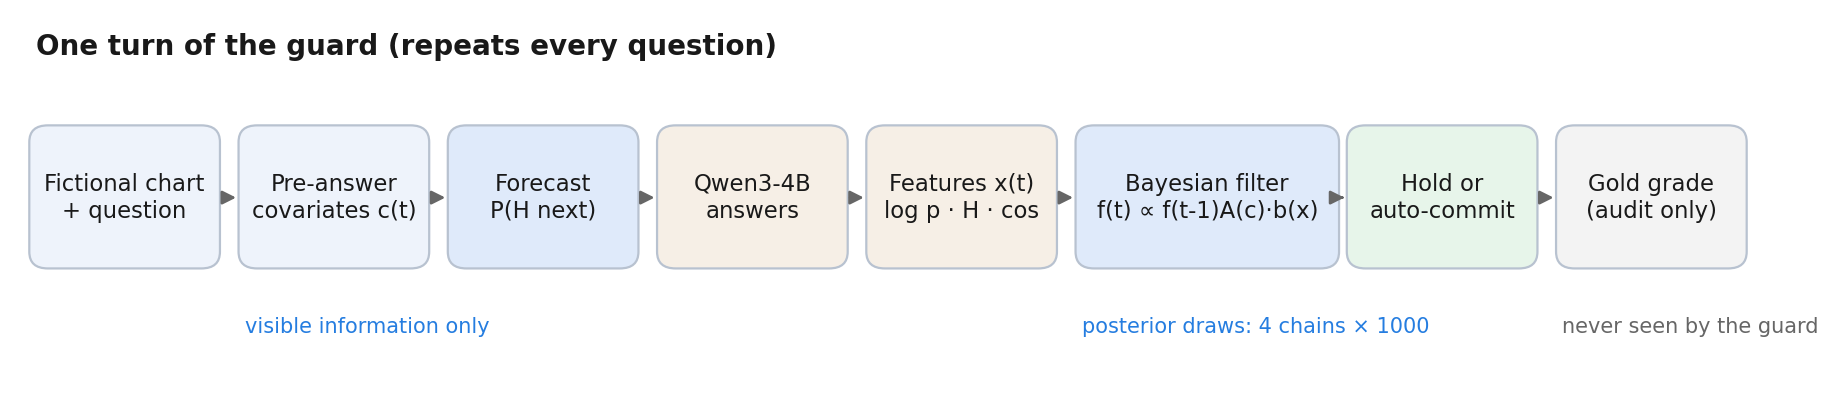
\includegraphics[width=\columnwidth]{pipeline.png}
\caption{One turn of the guard. Covariates and the forecast use visible information only; the gold grade is used solely for evaluation.}
\label{fig:pipe}\end{figure}

\section{Priors and Bayesian Inference}
\textbf{Priors} (Fig.~\ref{fig:priors}; standardised features). $\pi\sim\mathrm{Dir}(1,1,1)$; $A_{i\cdot}\sim\mathrm{Dir}(1+\kappa\mathbf 1[i{=}j])$ with $\kappa=0$, and $\kappa=2,5$ as a sensitivity analysis because a sticky prior can manufacture persistence; $w_j\sim\mathrm{Dir}(1,1)$; $v\sim\mathrm{InvGamma}(3,2)$ (prior mean 1); $\mu\mid v\sim\mathcal N(0,v/0.5)$. For M4: $\alpha\sim\mathcal N(0,1.5^2)$, $\beta_{ij,k}\sim\mathcal N(0,\sigma_k^2)$, $\sigma_k\sim\mathrm{HalfNormal}(0.5)$. These are weakly informative, shrink poorly supported covariate effects, and imply a broad prior on $P(\text{next}=H)$.

\textbf{Conjugate Gibbs with FFBS (M3).} Hidden paths are drawn jointly per dossier by forward filtering and backward sampling, $p(z_t{=}i\mid z_{t+1}{=}j)\propto f_t(i)A_{ij}$. Mixture indicators are drawn given the paths. The parameters then have conjugate conditionals: Dirichlet for $\pi$, $A$ and $w$, and Normal--Inverse-Gamma for each $(\mu,v)$.

\textbf{Metropolis-within-Gibbs (M4).} Given the paths, each origin's logit block is a multinomial-logistic regression. It is updated by random-walk MH with a Laplace-shaped proposal that adapts only during warm-up. Each $\log\sigma_k$ gets its own MH step with the Jacobian included. NUTS was unavailable on Python 3.14; the target posterior is the same.

\textbf{Label switching.} Draws are aligned to an EM reference by state-mean signatures and then re-mapped to G/U/H on validation labels.

\textbf{Prediction.} Filtered risk is averaged over 200 posterior draws (a frozen ensemble). An importance-reweighted variant weights each draw by $p(x_{1:t}\mid\theta_s)$.

\textbf{Validation of inference.} The suite includes: exact enumeration of all $3^5$ paths (likelihood, marginals, pair marginals, Viterbi); a test of the FFBS sampling law; rank-normalised split $\widehat R$ and bulk/tail ESS~\cite{vehtari2021} with gate $\widehat R\le1.01$, ESS $\ge400$; simulation-based calibration (SBC)~\cite{talts2018}; and posterior predictive checks.

\textbf{Decisions.} A hold is issued when $P(H)>C_{FP}/(C_{FP}+C_{FN})=1/11$ (cost ratio 10). Intervention contrasts use a Bayesian bootstrap over prefixes, supplemented by exact sign tests.

\begin{figure*}[t]\centering
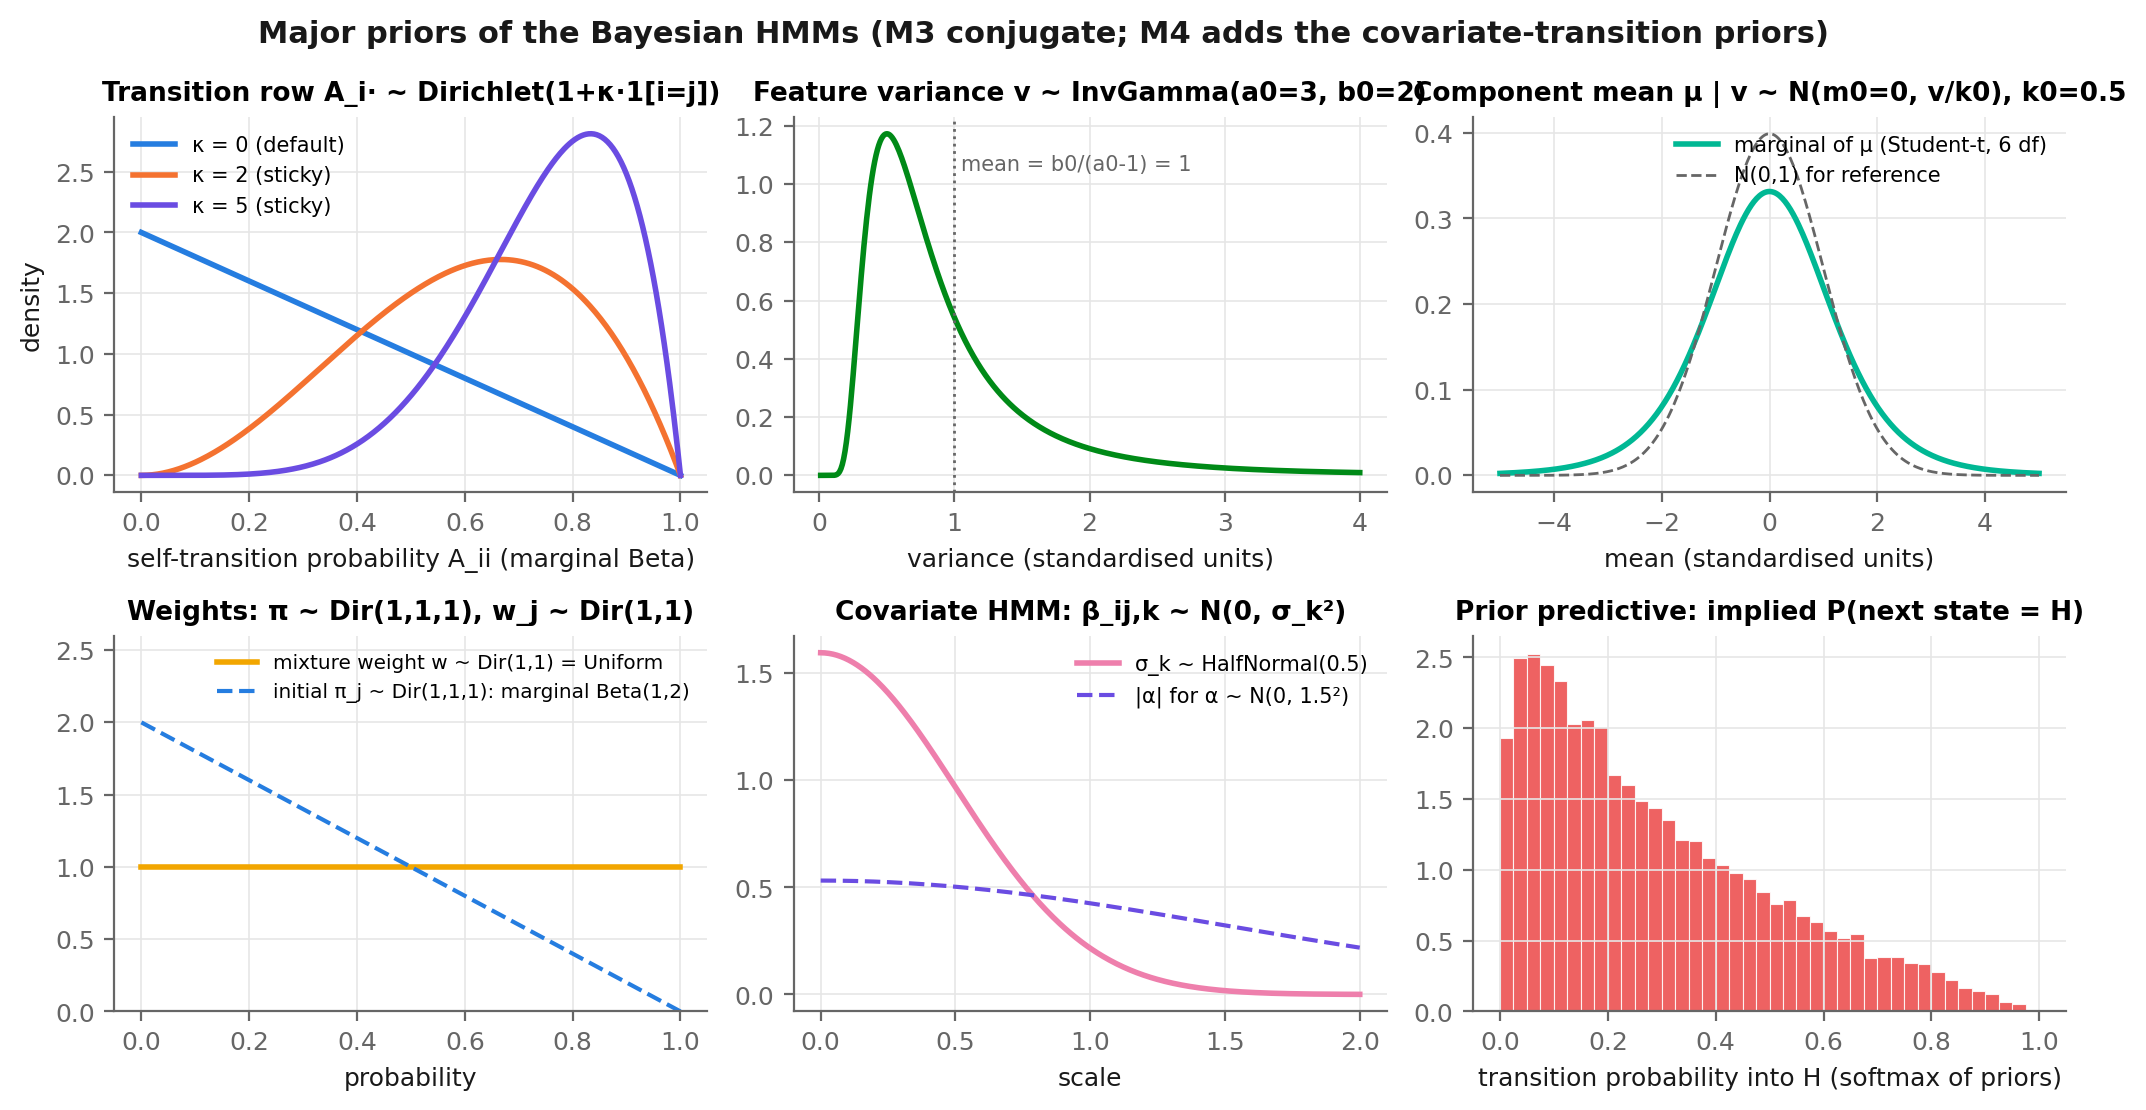
\includegraphics[width=.92\textwidth]{priors.png}
\caption{Major priors and the prior predictive transition probability into H implied by the covariate-transition priors.}
\label{fig:priors}\end{figure*}

\section{Experimental Protocol}
Splits are whole dossiers: 300/100/100 (registry) and 180/60/60 (clinical), fixed before fitting. Mappings and thresholds are frozen on validation, and the test set is opened once. The primary endpoint is first-onset detection: turns up to and including the first H. Differences use a whole-dossier paired bootstrap (2000 replicates). The locked analysis uses raw features with $M{=}2$. A post hoc exploratory analysis uses a fixed log-surprisal transform with $M{=}1$, because Qwen's confidence features are near point masses. Bayesian results come from 4 chains $\times$ (1000 warm-up $+$ 1000 draws).

\section{Results}
\begin{table}[t]\centering\small
\caption{First-onset detection on the test set (AUROC [95\% CI]). Registry, exploratory model set, corrected sampler.}
\begin{tabular}{lc}\toprule
Model & AUROC \\\midrule
M0 single feature & \AucMzeroRegX \\
M1 matched static & \AucMoneRegX \\
M2 EM-HMM filter & \AucMtwoRegX \\
M3 Bayesian HMM & \AucMthreeRegX \\
M4 covariate Bayes$^{\dagger}$ & \AucMfourRegX \\\bottomrule
\multicolumn{2}{l}{\footnotesize $^{\dagger}$fails the convergence gate ($\widehat R=\RhatMfourRegX$); provisional.}
\end{tabular}\label{tab:auc}\end{table}

\textbf{H1: history.} No measurable gain. The paired onset-AUROC difference (M2 $-$ M1) is \PrimRegL{} (registry, locked), \PrimRegX{} (registry, exploratory) and \PrimClinL{} (clinical, locked; \OnsetsClinL{} test onsets). The answer's own features dominate, and the filtered risk saturates near 0 or 1.

\textbf{H2: persistence.} The locked test, which permutes labels within turn and question type, finds clustering (\HtwoObsRegL{} H$\to$H vs.\ null \HtwoNullRegL{}, $p=\HtwoPRegL$). An exact count-preserving within-dossier null does not reject: $p=\WithinPRegL$ (registry), $p=\WithinPClinL$ (clinical). That null assumes exchangeable positions; a position-only control rejects ($p=\PosOnlyP$). Persistence beyond dossier difficulty and turn conditions is therefore neither established nor excluded (Fig.~\ref{fig:h2}).

\textbf{H3: risk factors} (association, M4). When the requested record is present, the risk of entering H from G changes by \EvidRegX{} (registry). Ambiguity changes it by \AmbRegX{} ($P{>}0=\AmbPRegX$).

\textbf{H4: forecasting.} Parameter integration (M3) changes the next-turn Brier score relative to plug-in EM by \BrierMthreeRegX{} on registry and \BrierMthreeClinX{} on clinical. No model beats a constant base rate.

\textbf{H5: randomised correction.} After a verified wrong answer, replacing it with the correct one lowered the next-turn H rate from \OrigHReg\% to \CorrHReg\% (registry, $n=\IvNReg$ prefixes). The risk difference is \CorrReg{} (\CorrBetterReg{} prefixes better, \CorrWorseReg{} worse, sign test $p=\CorrSignReg$); clinical: \CorrClin{}. A re-grounding reminder is weaker (\RegrReg{}) and raises unwarranted \texttt{UNKNOWN} answers by \RegrUReg.

\begin{figure}[t]\centering
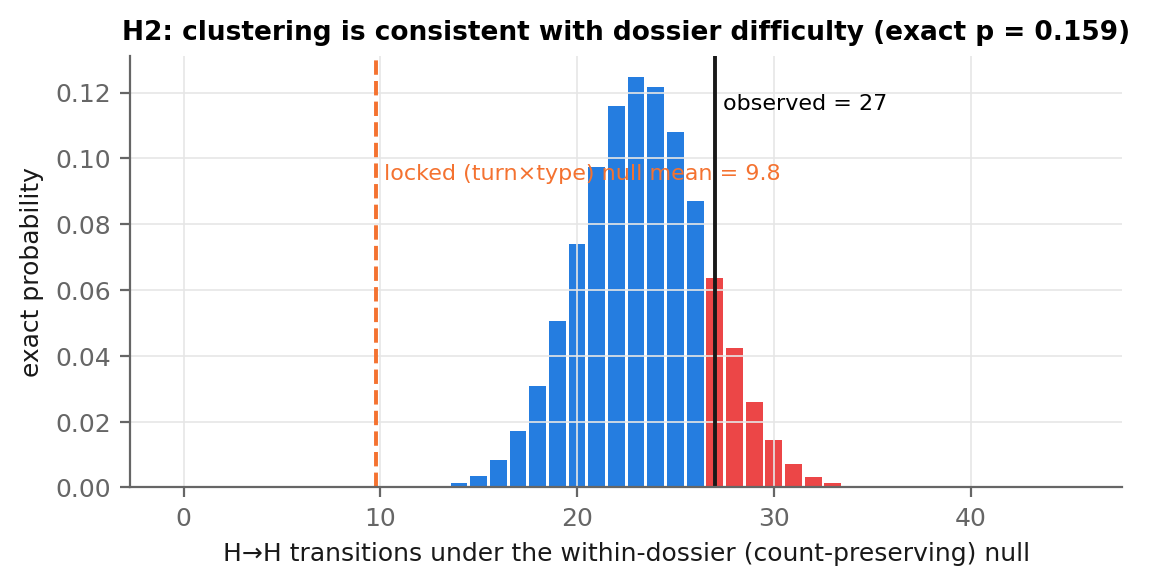
\includegraphics[width=\columnwidth]{h2_null.png}
\caption{Exact within-dossier null distribution of H$\to$H transitions (registry).}
\label{fig:h2}\end{figure}

\textbf{Application: clinical guard.} On 50 held-out fictional charts with paired seeds, holding answers when $P(H)>\GuardThr$ reduced silent errors from \GuardSilentU\% to \GuardSilentG\% of answers (\GuardHHeld/\GuardHtot{} errors held; hold rate \GuardHoldRate\%; precision \GuardPrec). Pre-emptive re-grounding did not reduce errors (paired difference \GuardPaired). The monitor-only policy caught \GuardMonCaught/\GuardMonTotal{} errors with \GuardMonHolds{} holds and is recommended.

\textbf{Red team.} Indirect prompt injection raised the H rate from \AtkClean\% to \AtkInj\%; the model obeyed the planted instruction \AtkObey{} times. Sycophancy pressure raised it to \AtkPressed\% on pressured turns. Ranking held (M4 onset AUROC \AtkAucInj{} under injection), but a 5\% false-stop alarm caught no onsets.

\begin{figure}[t]\centering
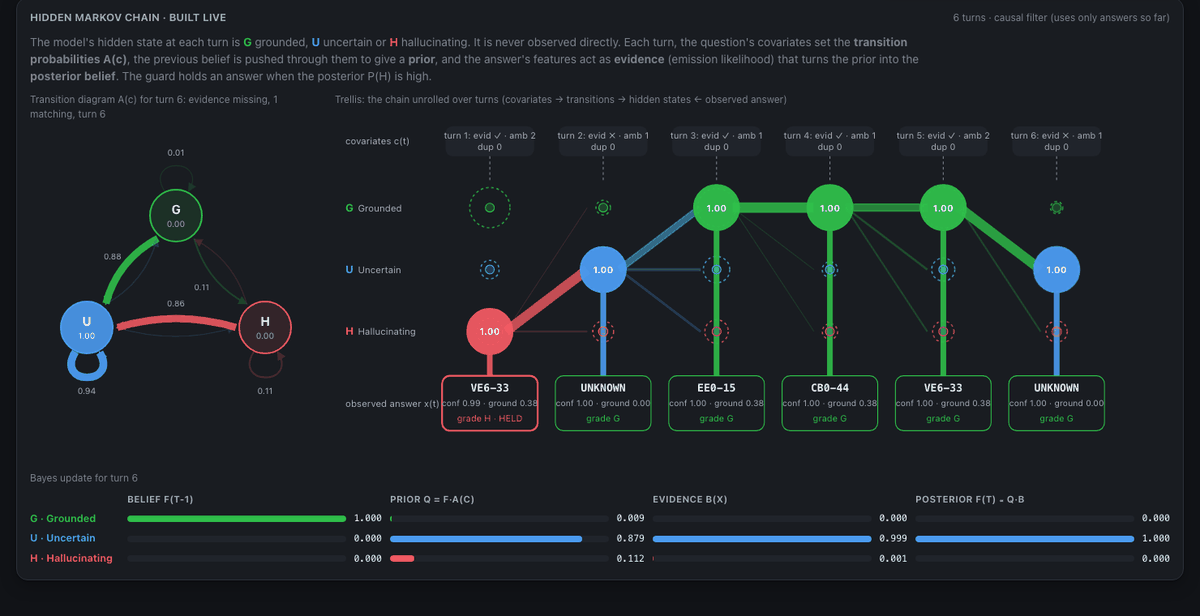
\includegraphics[width=\columnwidth]{demo_markov_chain_final.png}
\caption{The interactive UI building the hidden Markov chain for one chart (\S\ref{sec:review}).}
\label{fig:ui}\end{figure}

\section{Adversarial Review}\label{sec:review}
Every finding was reproduced independently before any change was made, and a change was adopted only on unanimous acceptance, under explicit anti-reward-hacking rules: no endpoint changes after test access, and no weakening of gates. The review found that the Gibbs variance step shared one Gamma draw across features. After the fix and an identical-configuration re-run, the EM results reproduced exactly and the exploratory M3 converged ($\widehat R$ \RhatPreMthreeRegX$\to$\RhatMthreeRegX, ESS \EssMthreeRegX). The SBC statistic for the maximum state mean moved from $p=\SbcPre$ to $p=\SbcPost$, and the independent-scenario coverage from \CovPre{} to \CovPost. The review also corrected an overstated persistence claim (H2) and documented an audit of the predecessor starter code. That starter's thresholds produced \StarterFS\% clean false stops, and its sampler had $\widehat R=\StarterRhat$.

\section{Limitations}
The task is fictional, uses short codes and a single quantised 4B checkpoint, and measures entropy through a top-20 proxy. The clinical test split has only \OnsetsClinL{} onsets. M4 and all two-component Bayesian fits still fail the convergence gate, so H3 is provisional. The state posterior is not a calibrated error probability: alarms under a 5\% false-stop budget never fire. The exploratory analyses were chosen after the locked results were seen.

\section{Conclusion}
History-based HMM filtering does not improve first-hallucination detection over a matched static detector here, because each answer's own signal dominates. What helps is knowing \emph{before} the answer whether the evidence exists, and correcting errors so they do not snowball. A Bayesian guard that holds risky answers reduced silent errors in a clinical setting. Its value comes from honest uncertainty reporting, not from temporal persistence.

\begin{thebibliography}{99}\footnotesize
\bibitem{rabiner1989} L.~R. Rabiner, ``A tutorial on hidden Markov models and selected applications in speech recognition,'' \emph{Proc. IEEE}, 1989.
\bibitem{bengio1995} Y.~Bengio and P.~Frasconi, ``An input output HMM architecture,'' \emph{NeurIPS}, 1994; \emph{IEEE Trans. Neural Netw.}, 1996.
\bibitem{zhang2024} M.~Zhang \emph{et al.}, ``How language model hallucinations can snowball,'' \emph{ICML}, 2024.
\bibitem{laban2025} P.~Laban, H.~Hayashi, Y.~Zhou, J.~Neville, ``LLMs get lost in multi-turn conversation,'' arXiv:2505.06120, 2025.
\bibitem{halluhard2026} ``HalluHard: a multi-turn hallucination benchmark,'' arXiv:2602.01031, 2026.
\bibitem{spikescore2026} ``Beyond in-domain detection: SpikeScore for cross-domain hallucination detection,'' arXiv:2601.19245, 2026.
\bibitem{diahalu2024} ``DiaHalu: a dialogue-level hallucination evaluation benchmark,'' arXiv:2403.00896, 2024.
\bibitem{farquhar2024} S.~Farquhar \emph{et al.}, ``Detecting hallucinations in large language models using semantic entropy,'' \emph{Nature}, 2024.
\bibitem{kossen2024} J.~Kossen \emph{et al.}, ``Semantic entropy probes,'' arXiv:2406.15927, 2024.
\bibitem{chuang2024} Y.-S. Chuang \emph{et al.}, ``Lookback Lens,'' \emph{EMNLP}, 2024.
\bibitem{mohri2024} C.~Mohri and T.~Hashimoto, ``Language models with conformal factuality guarantees,'' \emph{ICML}, 2024.
\bibitem{holsclaw2017} T.~Holsclaw \emph{et al.}, ``Bayesian non-homogeneous Markov models via P\'olya-gamma data augmentation,'' \emph{Ann. Appl. Stat.}, 2017.
\bibitem{pal2023} A.~Pal, L.~K. Umapathi, M.~Sankarasubbu, ``Med-HALT,'' \emph{CoNLL}, 2023.
\bibitem{kalai2025} A.~T. Kalai \emph{et al.}, ``Why language models hallucinate,'' arXiv:2509.04664, 2025.
\bibitem{vehtari2021} A.~Vehtari \emph{et al.}, ``Rank-normalization, folding, and localization: an improved $\widehat R$,'' \emph{Bayesian Anal.}, 2021.
\bibitem{talts2018} S.~Talts \emph{et al.}, ``Validating Bayesian inference algorithms with simulation-based calibration,'' arXiv:1804.06788, 2018.
\end{thebibliography}
\end{document}
